Wer die täglichen Änderungen eines Kontostands addiert, erhält die
Änderung zwischen Anfang und Ende. Die Zwischenstände fallen heraus.
Das ist die Teleskopformel. Werden die einzelnen Änderungen verschieden
gewichtet, fallen die Zwischenstände nicht mehr ganz heraus:
Neben einem Randbeitrag bleiben Beiträge an den Stellen, an denen sich
das Gewicht ändert.
Das ist die Abelsche partielle Summation.

Diese Lesefassung erläutert und beweist \GuideLink{} vollständig.
Wie die \NewtonLink{} führt sie von konkreten Rechnungen zu den
tragenden Identitäten. Am Ende werden die Bausteine für spätere kurze
Beweistabellen gebündelt. Die Gleichungsmarken (T), (A) und so weiter
sind lokale Orientierungshilfen; die Satznummer im Leitfaden bleibt
maßgeblich. Alle Summen im Hauptsatz sind endlich.

\section{Von Änderungen zu Zwischenständen}

Die Kontostände seien $10,13,11,15,12$. Die Änderungen sind
$3,-2,4,-3$. Deshalb gilt
\[
 (13-10)+(11-13)+(15-11)+(12-15)=12-10=2.
\]
Jeder innere Kontostand tritt einmal mit Plus und einmal mit Minus auf.
Nur die beiden Randwerte bleiben. Bei vielen Summanden ist daher die
entscheidende Frage: \emph{Kann ich jeden Summanden als Änderung
zweier benachbarter Werte schreiben?}

Nun gewichten wir dieselben Änderungen, die früheren stärker als
die späteren. Dazu schreiben wir $a_0=3$, $a_1=-2$, $a_2=4$ und
$a_3=-3$. Der kleine Buchstabe $a_k$ bezeichnet eine einzelne Änderung;
der große Buchstabe $A_k$ bezeichnet die \emph{Summe aller Änderungen
von der ersten bis zu dieser Stelle}:
\[
 \begin{aligned}
 A_0&=a_0=3, & A_1&=a_0+a_1=3-2=1,\\
 A_2&=a_0+a_1+a_2=3-2+4=5,
 & A_3&=a_0+a_1+a_2+a_3=3-2+4-3=2.
 \end{aligned}
\]
Weil wir bei $0$ zu zählen beginnen, enthält $A_0$ bereits die erste
Änderung. Die Zahlen $A_0,A_1,A_2,A_3$ geben hier also an, um wie viel
der jeweilige Kontostand nach einer, zwei, drei oder vier Buchungen
über dem Anfangswert $10$ liegt. Sie sind die \emph{Änderungen gegenüber
dem Anfang}, nicht die Kontostände $13,11,15,12$ selbst.

Wir wählen die Gewichte $b_0=8$, $b_1=6$, $b_2=3$, $b_3=1$:
\begin{center}
\begin{tabular}{@{}lrrrr@{}}
\toprule
Index $k$ & $0$ & $1$ & $2$ & $3$\\
\midrule
Änderung $a_k$ & $3$ & $-2$ & $4$ & $-3$\\
Partialsumme $A_k$ & $3$ & $1$ & $5$ & $2$\\
Gewicht $b_k$ & $8$ & $6$ & $3$ & $1$\\
\bottomrule
\end{tabular}
\end{center}
Direktes Ausrechnen gibt
\[
 8a_0+6a_1+3a_2+a_3=3\cdot8-2\cdot6+4\cdot3-3\cdot1=21.
\]

\subsection*{Warum zerlegen wir die Gewichte in Schichten?}

Unser Ziel ist, die gewichtete Summe durch die \emph{bereits
angesammelten Änderungen} $A_j$ auszudrücken. In ihnen sind positive
und negative Beiträge schon miteinander verrechnet: Beispielsweise
ist $A_1=3-2=1$, obwohl die beiden einzelnen Änderungen die Beträge
$3$ und $2$ haben. Um solche Ausgleichungen später beim Abschätzen
zu nutzen, wollen wir ganze Anfangsstücke gemeinsam gewichten.

Dazu stellen wir uns die Gewichte $8,6,3,1$ als vier nebeneinanderstehende
Säulen vor. Statt jede Säule einzeln zu betrachten, schneiden wir sie
\emph{waagerecht in Schichten}. Die unterste Schicht reicht von Höhe
$0$ bis Höhe $1$ und ist in allen vier Säulen vorhanden. Sie gewichtet
also alle vier Änderungen einmal und trägt
$a_0+a_1+a_2+a_3=A_3$ bei. Die nächste Schicht reicht von Höhe $1$
bis Höhe $3$: Sie hat Dicke $2$ und liegt nur in den ersten drei
Säulen. Ihr Beitrag ist deshalb $2(a_0+a_1+a_2)=2A_2$.
Entsprechend folgen eine Schicht der Dicke $3$ in den ersten beiden
Säulen und eine Schicht der Dicke $2$ nur in der ersten Säule.

% Vier Gewichte, zerlegt in gemeinsame horizontale Schichten.
% Vektorgrafik: Säulenhöhen sind b_k, Beschriftungen rechts sind Summenbeiträge.
\begin{center}
\begin{minipage}{\linewidth}
\centering
\definecolor{abelLayerOne}{HTML}{DCEAF3}
\definecolor{abelLayerTwo}{HTML}{B8D9D3}
\definecolor{abelLayerThree}{HTML}{E7C995}
\definecolor{abelLayerFour}{HTML}{BDB3D0}
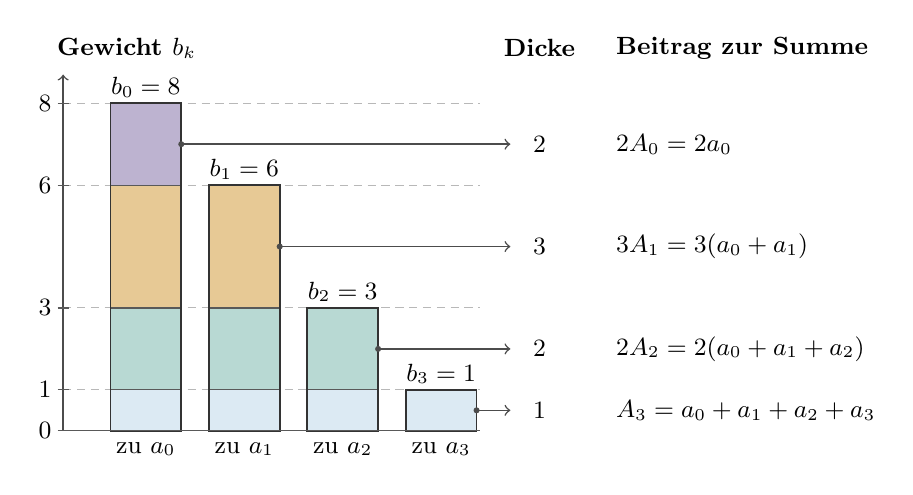
\begin{tikzpicture}[x=1cm,y=.52cm,font=\small,
  layer edge/.style={draw=black!65,line width=.45pt},
  guide/.style={draw=black!28,densely dashed,line width=.35pt},
  contribution/.style={draw=black!70,->,line width=.55pt}]
  % Höhenraster; die ausgefüllten Säulen liegen davor.
  \foreach \height in {1,3,6,8}
    \draw[guide] (0,\height) -- (5.3,\height);
  % Gemeinsame Schichten von unten nach oben.
  \foreach \left in {.6,1.85,3.1,4.35}
    \path[fill=abelLayerOne,layer edge] (\left,0) rectangle +(0.9,1);
  \foreach \left in {.6,1.85,3.1}
    \path[fill=abelLayerTwo,layer edge] (\left,1) rectangle +(0.9,2);
  \foreach \left in {.6,1.85}
    \path[fill=abelLayerThree,layer edge] (\left,3) rectangle +(0.9,3);
  \path[fill=abelLayerFour,layer edge] (.6,6) rectangle +(0.9,2);
  % Konturen und eindeutige Zuordnung zu den Änderungen a_k.
  \foreach \left/\height/\index in {.6/8/0,1.85/6/1,3.1/3/2,4.35/1/3} {
    \draw[black!80,line width=.65pt] (\left,0) rectangle +(0.9,\height);
    \node[above,inner sep=2pt] at ({\left+.45},\height)
      {$b_{\index}=\height$};
    \node[below,inner sep=4pt] at ({\left+.45},0) {zu $a_{\index}$};
  }
  \draw[->,black!70,line width=.55pt] (0,0) -- (0,8.7);
  \draw[black!65,line width=.45pt] (0,0) -- (5.3,0);
  \foreach \height in {0,1,3,6,8} {
    \draw[black!65] (-.07,\height) -- (.07,\height);
    \node[left,inner sep=4pt] at (0,\height) {$\height$};
  }
  \node[anchor=west,font=\small\bfseries] at (-.2,9.35) {Gewicht $b_k$};
  \node[font=\small\bfseries] at (6.05,9.35) {Dicke};
  \node[anchor=west,font=\small\bfseries] at (6.9,9.35) {Beitrag zur Summe};
  % Verbindungen jeweils vom rechten Ende der gesamten Schicht.
  \foreach \right/\middle/\thickness in {5.25/.5/1,4/2/2,2.75/4.5/3,1.5/7/2} {
    \fill[black!70] (\right,\middle) circle[radius=1.1pt];
    \draw[contribution] (\right,\middle) -- (5.68,\middle);
    \node at (6.05,\middle) {$\thickness$};
  }
  \node[anchor=west] at (6.9,.5)
    {$\boldsymbol{A_3}=a_0+a_1+a_2+a_3$};
  \node[anchor=west] at (6.9,2)
    {$\boldsymbol{2A_2}=2(a_0+a_1+a_2)$};
  \node[anchor=west] at (6.9,4.5)
    {$\boldsymbol{3A_1}=3(a_0+a_1)$};
  \node[anchor=west] at (6.9,7)
    {$\boldsymbol{2A_0}=2a_0$};
\end{tikzpicture}
\par\smallskip
{\small\raggedright
Die Säulen zeigen die Gewichte $b_k$. Gleichfarbige Teile bilden
zusammen eine waagerechte Schicht und gewichten ein Anfangsstück
der Änderungen $a_k$. Rechts steht der Beitrag der \emph{ganzen}
Schicht zur gewichteten Summe.\par}
\end{minipage}
\end{center}


Dieselbe Zerlegung lässt sich auch als Tabelle lesen:
\begin{center}
\begin{tabular}{@{}lrrrrl@{}}
\toprule
Schicht & bei $a_0$ & bei $a_1$ & bei $a_2$ & bei $a_3$ & Beitrag\\
\midrule
von $0$ bis $1$ & $1$ & $1$ & $1$ & $1$ & $A_3$\\
von $1$ bis $3$ & $2$ & $2$ & $2$ & $0$ & $2A_2$\\
von $3$ bis $6$ & $3$ & $3$ & $0$ & $0$ & $3A_1$\\
von $6$ bis $8$ & $2$ & $0$ & $0$ & $0$ & $2A_0$\\
\midrule
Gewicht insgesamt & $8$ & $6$ & $3$ & $1$ &\\
\bottomrule
\end{tabular}
\end{center}
\Needspace{12\baselineskip}
Die Einträge geben an, wie viel Gewicht die jeweilige Schicht zu
jedem $a_k$ beiträgt. Liest man die Tabelle \emph{spaltenweise}, erhält
man wieder die ursprünglichen Gewichte, etwa $1+2+3+2=8$ bei $a_0$.
Liest man sie \emph{zeilenweise}, erhält man die gewichteten
Anfangsstücke. Es wird also nichts an der Summe geändert, sondern
nur anders zusammengefasst:
\begin{align*}
 8a_0+6a_1+3a_2+a_3
 &=(a_0+a_1+a_2+a_3)+2(a_0+a_1+a_2)\\
 &\quad +3(a_0+a_1)+2a_0\\
 &=A_3+2A_2+3A_1+2A_0\\
 &=2+10+3+6=21.
\end{align*}
Weil die Säulen von links nach rechts niedriger werden, erfasst jede
Schicht genau ein Anfangsstück. Deshalb erscheinen gerade die
Partialsummen $A_j$. Die Schichtdicken sind das letzte Gewicht $1$
und die Abnahmen $3-1$, $6-3$, $8-6$. Das erklärt die Abelsche Formel:
\emph{Einzelglieder mit Gewichten werden zu Partialsummen mit
Gewichtsänderungen.} Für längere Folgen können die Partialsummen
klein bleiben, obwohl viele einzelne Beiträge auftreten. Die
Schichtenzerlegung bewahrt diese Ausgleichung, bevor wir Beträge
bilden und abschätzen.

\Needspace{10\baselineskip}
\section{Die genaue Aussage}

Wir verwenden $\N=\{0,1,2,\ldots\}$ und reelle Folgen.
Seien $r,s\in\N$ mit $r\leq s$. Eine Summe über ein leeres
Indexintervall hat den Wert $0$.

\textbf{Teleskopformel.} Für jede reelle Folge $u$ gilt
\begin{equation}\tag{T}\label{abel:telescoping}
 \boxed{\displaystyle
 \sum_{k=r}^{s}(u_{k+1}-u_k)=u_{s+1}-u_r.}
\end{equation}
Die Summe der Änderungen ist die Änderung zwischen den Randwerten.
Mit $(\Delta u)_k=u_{k+1}-u_k$ heißt das auch:
Summieren macht das Differenzieren bis auf den Anfangswert rückgängig.

\textbf{Abelsche Summationsformel.} Für reelle Folgen $a,b$ setze
\[
 A_j=\sum_{k=r}^{j}a_k\qquad(r\leq j\leq s).
\]
Dann gilt
\begin{equation}\tag{A}\label{abel:summation}
 \boxed{\displaystyle
 \sum_{k=r}^{s}a_kb_k
 =A_sb_s+\sum_{k=r}^{s-1}A_k(b_k-b_{k+1}).}
\end{equation}
Hier sind die Partialsummen ausdrücklich \emph{ab $r$} gebildet.
Der erste Term rechts ist der Randbeitrag; die übrigen Terme
berücksichtigen die Änderungen der Gewichte. Die Identität gilt
auch für negative oder nichtmonotone Gewichte.

\textbf{Abschätzung.} Gilt zusätzlich für ein $C\geq0$
\[
 |A_j|\leq C\quad(r\leq j\leq s),\qquad
 b_r\geq b_{r+1}\geq\cdots\geq b_s\geq0,
\]
so folgt
\begin{equation}\tag{E}\label{abel:estimate}
 \boxed{\displaystyle
 \left|\sum_{k=r}^{s}a_kb_k\right|\leq Cb_r.}
\end{equation}
Die Schranke hängt von der größten zugelassenen Auslenkung der
Partialsumme und vom ersten Gewicht ab, nicht von der Anzahl der
Summanden. Für $r=s$ wird (A) zu $a_rb_r=A_rb_r$; ihre zweite
Summe ist leer. Konvergenzannahmen sind in keinem der drei Teile nötig.

\section{Der kurze Beweiskern}

\subsection*{1. Teleskopieren: die inneren Werte heben sich auf}

In
\[
 (u_{r+1}-u_r)+(u_{r+2}-u_{r+1})+\cdots+(u_{s+1}-u_s)
\]
heben sich alle inneren Werte auf; es bleibt $u_{s+1}-u_r$.
Formal genügt Induktion über die Anzahl der Summanden:
Der erste Schritt ist $u_{r+1}-u_r$; das Anhängen von
$u_{s+2}-u_{s+1}$ ersetzt den Endwert $u_{s+1}$ durch $u_{s+2}$.
Damit ist (T) bewiesen.

\subsection*{2. Abel: ein Produkt teleskopieren}

Aus $A_r=a_r$ und $A_{k+1}-A_k=a_{k+1}$ folgt für $r\leq k<s$
durch Ausmultiplizieren die einzige benötigte Produktidentität:
\begin{equation}\tag{P}\label{abel:product}
 a_{k+1}b_{k+1}
 =\underbrace{A_{k+1}b_{k+1}-A_kb_k}_{\text{Änderung des Produkts}}
   +A_k(b_k-b_{k+1}).
\end{equation}
Summieren und (T) auf die Produkte $A_kb_k$ anwenden liefert
\[
 \sum_{k=r+1}^{s}a_kb_k
 =A_sb_s-A_rb_r+\sum_{k=r}^{s-1}A_k(b_k-b_{k+1}).
\]
Nun auf beiden Seiten $a_rb_r=A_rb_r$ addieren: Das ist (A).
Für $r=s$ gilt die Formel unmittelbar. Ein künstlicher Index $r-1$
ist nicht nötig; der Beweis gilt daher auch bei $r=0$ unverändert.

\subsection*{3. Die Abschätzung: die Gewichtsabnahmen addieren sich}

Alle Zahlen $b_s$ und $b_k-b_{k+1}$ sind nichtnegativ. Deshalb ergibt
(A) mit der Dreiecksungleichung
\begin{align*}
 \left|\sum_{k=r}^{s}a_kb_k\right|
 &\leq |A_s|b_s+\sum_{k=r}^{s-1}|A_k|(b_k-b_{k+1})\\
 &\leq C\left(b_s+\sum_{k=r}^{s-1}(b_k-b_{k+1})\right)
  =Cb_r.
\end{align*}
Die letzte Gleichheit ist wieder Teleskopieren. Das beweist (E)
und damit das ganze Theorem. Für $r=s$ ist die Klammer einfach $b_r$.

\section{Warum die Abschätzung so gut passt}

Die Schichten aus dem Eingangsbeispiel erklären auch die Konstante.
Für $b_r>0$ sind
\[
 \frac{b_s}{b_r}\quad\text{und}\quad
 \frac{b_k-b_{k+1}}{b_r}\quad(r\leq k<s)
\]
nichtnegative Gewichte, deren Summe $1$ ist. Nach (A) ist daher
$\bigl(\sum_{k=r}^{s}a_kb_k\bigr)/b_r$ ein \emph{gewichteter
Mittelwert} der Partialsummen $A_r,\ldots,A_s$.
Liegen alle diese Zahlen zwischen $-C$ und $C$, dann auch ihr
gewichteter Mittelwert. Für $b_r=0$ sind sämtliche Gewichte $b_k=0$,
also ist die Aussage unmittelbar.

Im Eingangsbeispiel ist $C=5$. Die Abschätzung ergibt $|21|\leq5\cdot8=40$.
Sie soll den Wert nicht exakt ausrechnen, sondern ihn ohne Kenntnis
aller Einzelheiten kontrollieren. Die Konstante $1$ vor $Cb_r$ lässt
sich allgemein nicht verbessern: Bei $a_r=C$ und $a_k=0$ für $k>r$
gilt $A_j=C$ und die gewichtete Summe ist genau $Cb_r$.

Ohne monotone Gewichte liefert dieselbe Rechnung immerhin
\begin{equation}\tag{V}\label{abel:variation}
 \left|\sum_{k=r}^{s}a_kb_k\right|
 \leq C\left(|b_s|+\sum_{k=r}^{s-1}|b_k-b_{k+1}|\right).
\end{equation}
Der Ausdruck in der Klammer misst den Endwert und die gesamte
Bewegung der Gewichte. Bei fallenden nichtnegativen Gewichten ist er
exakt $b_r$. Diese Zusatzformel erklärt, was an der Monotonie gebraucht
wird; sie ist kein weiterer Baustein für den Hauptbeweis.

\section{Vier Anwendungen}

\subsection*{Eine Bruchsumme schrumpft auf zwei Randwerte}

Für $1\leq r\leq s$ gilt
\[
 \frac1{k(k+1)}=\frac1k-\frac1{k+1}.
\]
Mit $u_k=-1/k$ auf dem betrachteten positiven Indexbereich liefert (T)
sofort
\[
 \boxed{\displaystyle
 \sum_{k=r}^{s}\frac1{k(k+1)}=\frac1r-\frac1{s+1}.}
\]
Beispielsweise ist die Summe von $k=1$ bis $100$ genau $100/101$.
Das Finden der Differenz ist die eigentliche Idee; danach bleiben
nur Anfang und Ende. Falls man $u$ als Folge auf ganz $\N$ auffassen
möchte, kann $u_0$ beliebig, etwa als $0$, ergänzt werden.

\subsection*{Anschluss an Newton: Summieren hebt den Basisindex}

Die \NewtonLink{} verwendet die Binomialfolgen $\binom nk$.
Aus der Pascal-Identität folgt für $n,k\in\N$
\[
 \binom nk=\binom{n+1}{k+1}-\binom n{k+1}.
\]
Dabei gilt $\binom nk=0$ für $k>n$. Teleskopieren gibt deshalb
\[
 \sum_{n=0}^{N-1}\binom nk=\binom N{k+1}\qquad(N\in\N).
\]
Für $N=0$ sind beide Seiten null. Differenzieren senkt in dieser Basis
den Index, Summieren hebt ihn. So wird aus
$n^2=\binom n1+2\binom n2$ unmittelbar
\[
 \sum_{n=0}^{N-1}n^2
 =\binom N2+2\binom N3
 =\frac{N(N-1)(2N-1)}6.
\]
Die Newtondarstellung liefert eine passende Darstellung der Summanden;
die Teleskopformel summiert deren Bestandteile.

\subsection*{Eine geometrische Summe mit wachsendem Faktor}

Gesucht ist $S_n=\sum_{k=0}^{n}kq^k$ für $q\in\R$, $q\ne1$.
Wir nehmen $a_k=q^k$, $b_k=k$. Die Partialsummen des ersten Faktors
sind einfach:
\[
 A_k=\frac{1-q^{k+1}}{1-q},\qquad b_k-b_{k+1}=-1.
\]
Damit liefert (A) für $n\geq1$
\begin{align*}
 S_n
 &=n\frac{1-q^{n+1}}{1-q}
   -\sum_{k=0}^{n-1}\frac{1-q^{k+1}}{1-q}\\
 &=\frac{q-(n+1)q^{n+1}+nq^{n+2}}{(1-q)^2}.
\end{align*}
Für $n=0$ sind beide Seiten $0$; für $q=1$ erhält man stattdessen
$S_n=n(n+1)/2$. Wie üblich ist $q^0=1$, auch bei $q=0$.
Die wachsenden Gewichte sind hier erwünscht: Ihre Differenzen sind
konstant. Für eine Identität braucht man keine Monotonieannahme wie
in (E). Man wählt den Faktor mit einfachen Partialsummen als $a_k$
und den mit einfachen Differenzen als $b_k$.

\subsection*{Vorzeichenwechsel: eine Summe bleibt klein}

Seien $1\leq r\leq s$ und $a_k=(-1)^k$. Auf jedem neu begonnenen
Indexintervall sind die Partialsummen $A_j$ entweder $0$ oder
$(-1)^r$. Es gilt also $|A_j|\leq1$. Mit den fallenden Gewichten
$b_k=1/k$ folgt aus (E)
\[
 \boxed{\displaystyle
 \left|\sum_{k=r}^{s}\frac{(-1)^k}{k}\right|\leq\frac1r.}
\]
Das ist bereits eine Aussage über \emph{jede endliche} Teilsumme.
Zum Beispiel ist der Betrag der Summe von $k=100$ bis $10000$
höchstens $1/100$. Die direkte Dreiecksungleichung ergäbe dagegen
$\sum_{k=100}^{10000}1/k$, eine Zahl größer als $1$:
Schon die ersten $101$ dieser Summanden sind mindestens $1/200$,
die nächsten $200$ mindestens $1/400$.
Die Abelsche Umformung nutzt die gegenseitige Aufhebung der Vorzeichen,
bevor Beträge gebildet werden.

\section{Partielle Summation als diskrete partielle Integration}

Die Produktregel für Differenzen lautet
\[
 u_{k+1}v_{k+1}-u_kv_k
 =(u_{k+1}-u_k)v_{k+1}+u_k(v_{k+1}-v_k).
\]
Summieren von $r$ bis $s-1$ und Umstellen ergibt
\begin{equation}\tag{I}\label{abel:integration}
 \sum_{k=r}^{s-1}u_k(v_{k+1}-v_k)
 =u_sv_s-u_rv_r
  -\sum_{k=r}^{s-1}(u_{k+1}-u_k)v_{k+1}.
\end{equation}
Das entspricht der partiellen Integration
\[
 \int_\alpha^\beta u(x)v'(x)\,dx
 =[u(x)v(x)]_\alpha^\beta-\int_\alpha^\beta u'(x)v(x)\,dx
\]
für stetig differenzierbare Funktionen. Im diskreten Fall steht im
letzten Summanden allerdings $v_{k+1}$. Diese Verschiebung gehört zur
Produktregel und darf nicht entfallen. Die Abelsche Formel ist genau
diese Rechnung mit Partialsummen als diskreter Stammfunktion.
Der kurze Beweis von (A) hat sie bereits in der benötigten Form
verwendet; Differential- oder Integralrechnung setzt er nicht voraus.

\subsection*{Was für unendliche Reihen hinzukommt}

Die endliche Abschätzung erklärt auch das Dirichlet-Kriterium.
Seien die globalen Partialsummen $P_j=\sum_{k=0}^{j}a_k$ durch
$|P_j|\leq M$ für alle $j\in\N$ und ein $M\geq0$ beschränkt,
und sei $b_k$ eine fallende nichtnegative Nullfolge.
Für einen späteren Anfang $r\geq1$ gilt
\[
 A_j=P_j-P_{r-1},\qquad |A_j|\leq2M.
\]
Also ist nach (E) für jedes $s\geq r$
\[
 \left|\sum_{k=r}^{s}a_kb_k\right|\leq2Mb_r\longrightarrow0
 \quad(r\to\infty).
\]
Das Cauchy-Kriterium in $\R$ liefert die Konvergenz von
$\sum_{k=0}^{\infty}a_kb_k$. Erst hier kommen ein Grenzübergang und
die Vollständigkeit von $\R$ hinzu. Aus $|P_j|\leq M$ allein darf
man auf einem verschobenen Abschnitt nicht $|A_j|\leq M$ folgern;
das alternierende Beispiel hatte die stärkere Schranke $1$ direkt
für jedes Anfangsstück ab $r$ geliefert.

\section{Bausteine für möglichst kurze Beweistabellen}

Der Hauptsatz braucht weder Newtondarstellung noch geometrische
Summen, Integralrechnung oder einen Konvergenzsatz. Über der bereits
verfügbaren endlichen Summenrechnung genügen die folgenden Schritte:
\begin{center}
\small
\renewcommand{\arraystretch}{1.15}
\begin{tabularx}{\linewidth}{@{}p{.20\linewidth}X@{}}
\toprule
Baustein & Inhalt und Verwendung\\
\midrule
Summenrekursion &
$A_r=a_r$ und $A_{k+1}=A_k+a_{k+1}$; leere Summe $=0$.
Linearität und eine Verschiebung des Summationsindex.\\
Teleskopieren (T) &
Eine Induktion über die Intervalllänge; beim Anhängen eines Summanden
ändert sich nur der Endwert.\\
Produktidentität (P) &
$A_{k+1}-A_k=a_{k+1}$ einsetzen und ausmultiplizieren.
Eine lokale Gleichheit, keine eigene Induktion.\\
Abel (A) &
(P) summieren, (T) auf $A_kb_k$ anwenden,
$A_rb_r=a_rb_r$ ergänzen.\\
Abschätzung (E) &
Dreiecksungleichung, $|A_k|\leq C$, Nichtnegativität der
Gewichtsabnahmen und einmal (T).\\
\bottomrule
\end{tabularx}
\end{center}

Die Abhängigkeiten sind damit
\[
 \text{Summenrekursion}\ \longrightarrow\ \text{(T), (P)}
 \ \longrightarrow\ \text{(A)}\ \longrightarrow\ \text{(E)}.
\]
Für die Tabelle zu (A) reicht nach (P) eine einzige Summengleichung
mit Randkorrektur; eine zweite Induktion über die Abelsche Formel
ist nicht erforderlich. In der Tabelle zu (E) bleibt die oben
gezeigte Ungleichungskette erhalten. Die Summenregeln und die
Dreiecksungleichung werden, soweit noch nicht verfügbar, einmal als
Hilfssätze bereitgestellt.

Die Randfälle sollen sichtbar, aber kurz bleiben: $r=s$ wird direkt
erledigt; $r=0$ benötigt dank (P) keine negativen Indizes.
Die Abschätzung schließt $C=0$ und $b_r=0$ bereits ein, ohne durch
einen dieser Werte zu teilen. Die Mittelwertdeutung, die Beispiele
und (I) erklären den Satz, vergrößern aber seinen formalen Beweiskern
nicht. So kristallisieren sich drei Ideen heraus: \emph{innere Terme
aufheben, ein Produkt differenzieren, die verbleibenden Gewichte addieren.}
